%\documentclass[trans]{beamer}
\documentclass[9pt]{beamer}

% Try the class options [notes], [notes=only], [trans], [handout],
% [red], [compress], [draft], [class=article] and see what happens!

% Copyright 2003 by Till Tantau <tantau@users.sourceforge.net>.
%
% This program can be redistributed and/or modified under the terms
% of the LaTeX Project Public License Distributed from CTAN
% archives in directory macros/latex/base/lppl.txt.

% For a green structure color use:
%\colorlet{structure}{green!50!black}

%%%%%%%%%% User macros%%%%%%%%%%%
\newcommand{\mypurple}[1]{{\color[rgb]{0.7,0,0.8}#1}}
\newcommand{\myred}  [1] {{\color{red}#1}}
\newcommand{\myblue} [1] {{\color{blue}#1}}
\newcommand{\mygreen}[1] {{\color[rgb]{0,0.5,0}#1}}
\newcommand{\Nat}{\mathbb{N}}
\def\sla  {\!\!\!\slash}
%%%%%%%%%%%%%%%%%%%%%%%%%%%%%%%%%
\mode<article> % only for the article version
{
  \usepackage{beamerbasearticle}
  \usepackage{fullpage}
  \usepackage{hyperref}
}

%\beamertemplateshadingbackground{red!10}{blue!10}
%\beamertemplateshadingbackground{blue!10}{blue!10}

%\usepackage{beamerthemeshadow}

\usepackage{pgf,pgfarrows,pgfnodes,pgfautomata,pgfheaps,pgfshade}
\usepackage{amsmath,amssymb}
\usepackage[latin1]{inputenc}
\usepackage{colortbl}
\usepackage[english]{babel}
%\usepackage{verbatim}
%\usepackage{listings}
\usepackage[procnames]{listings}

%\usepackage{lmodern}
\usepackage[T1]{fontenc} 

\usepackage{times}

% for code colouring
\include{pythonlisting}
\include{cpplisting}

% Use some nice templates
\beamertemplatetransparentcovereddynamic
\usetheme{Binet}
%\usetheme{Madrid}
%\usetheme{Boadilla}
%\usetheme{Berkeley}
%\usetheme{Rochester}

%\def\command#1{\list{}{\leftmargin=2em\itemindent-\leftmargin\def\makelabel##1{\hss##1}}%
%\item\extractcommand#1@\par\topsep=0pt}
%\def\endcommand{\endlist}
%\def\extractcommand#1#2@{\strut\declare{\texttt{\string#1}}#2}

%
% The following info should normally be given in you main file:
%

\hypersetup{%
  pdftitle={AthenaMP},%
  pdfauthor={Sebastien Binet},
  pdfsubject={AthenaMP},
  pdfkeywords={ATLAS,Athena,multiprocess},
%  pdfpagemode=FullScreen%
}

\title[AthenaMP]{AthenaMP:\\Athena on steroids}
\author[S. Binet]{S\'ebastien~Binet}%\inst{1}
\institute[LAL]{
%  \inst{1}%
  Laboratoire \\de \\l'Acc\'el\'erateur Lin\'eaire}
\date{18-12-2008}

% \begin{center}
% On behalf of Core people
% \end{center}

\pgfdeclaremask{lal}{lal}
%\pgfdeclaremask{ubp}{UBP-logo}
\pgfdeclareimage[mask=lal,width=3cm]{lal-logo}{lal}
%\pgfdeclareimage[mask=ubp,width=1cm]{ubp-logo}{UBP-logo}

\logo{%
  \vbox{%
    \hbox{\hfil\pgfuseimage{lal-logo}}%
    %\vskip0.1cm%
    %\hbox{\pgfuseimage{ubp-logo}}%
  }%
}


\begin{document}
\lstset{language=C++}

\frame{\titlepage
%  \hskip0.44\paperwidth
%  \insertlogo

    \begin{beamercolorbox}[sep=8pt,center,fg]{mylogo}
      \usebeamercolor[fg]{mylogo}\insertlogo
    \end{beamercolorbox}

}

%\section*{Outline}
%\frame{\tableofcontents[part=1]}%,pausesections]}

%\AtBeginSubsection[]
%{
%  \frame<handout:0>
%  {
%    \frametitle{Outline}
%    \tableofcontents[current,currentsubsection]
%  }
%}

\part<presentation>{Main Talk}

%%%%%%%%%%%%%%%%%%%%%%%%%%%%%%%%%%%%%%%%%%%%%%%%%%%%%%%%%%%%%%%%%%%%%%%%%%%%%%%
%%%%%%%%%%%%%%%%%%%%%%%%%%%%%%%%%%%%%%%%%%%%%%%%%%%%%%%%%%%%%%%%%%%%%%%%%%%%%%%
%\section[Outline]{Outline}

% \frame<beamer>{
%   \frametitle{Outline}
%   \begin{columns}
% \begin{column}{0.49\textwidth}
%   \begin{block}{}
%   \tableofcontents
%   \end{block}
% \end{column}
% \end{columns}

% }
%\frame{\partpage}

%%%%%%%%%%%%%%%%%%%%%%%%%%%%%%%%%%%%%%%%%%%%%%%%%%%%%%%%%%%%%%%%%%%%%%%%%%%%%%%
%%%%%%%%%%%%%%%%%%%%%%%%%%%%%%%%%%%%%%%%%%%%%%%%%%%%%%%%%%%%%%%%%%%%%%%%%%%%%%%
\section[AthenaMP]{AthenaMP}

\frame{
  \frametitle{Motivations}

  \begin{columns}
    \begin{column}{0.9\textwidth}

      \begin{block}{\texttt{Athena}: fiche technique}
        \begin{itemize}
          \item \emph{framework} bas\'e sur \textsc{Gaudi}
          \item association de multiples composants \'el\'ementaires:
            \begin{itemize}
              \item \texttt{Algorithm, AlgTool, Service},\ldots
            \end{itemize}
          \item un seul fil d'execution (\emph{single thread})
          \item reconstruction (14.5.0):
            \begin{itemize}
              \item \texttt{rdotoesdnotrigger}:
                \begin{itemize}
                  \item $\sim 1.6\ Gb\ VMEM$
                  \item $\sim 10\ s/evt\ (\sim 24000\ kSi2k)$
                \end{itemize}
              \item \texttt{rdotoesd}:
                \begin{itemize}
                  \item $\sim 2.1\ Gb\ VMEM$
                  \item $\sim 15\ s/evt\ (\sim 37000\ kSi2k)$
                \end{itemize}
              \item \texttt{esdtoaod}:
                \begin{itemize}
                  \item $\sim 1.3\ Gb\ VMEM$
                  \item $\sim 1\ s/evt\ (\sim 2500\ kSi2k)$
                \end{itemize}
            \end{itemize}
        \end{itemize}
      \end{block}

    \end{column}
  \end{columns}

  \begin{figure}
    \begin{center}
      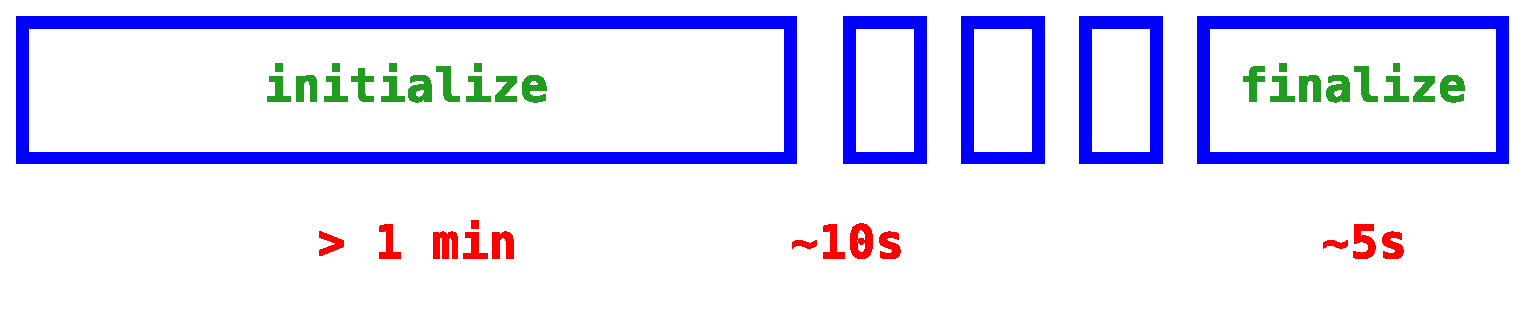
\includegraphics[angle=0,width=0.5\textwidth]{figs/athena-sequence.eps}
    \end{center}
  \end{figure}
}

\frame{
  \frametitle{Motivations - II}

  \begin{columns}
    \begin{column}{0.9\textwidth}

      \begin{block}{\emph{hardware}: tendance g\'en\'erale}
        \begin{itemize}
          \item $CPU \Rightarrow$ multicores
            \begin{itemize}
              \item chaque $CPU$ peut comporter plusieurs ($2\rightarrow\sim 1024$) unit\'es de calcul
            \end{itemize}
          \item chaque \emph{core} est moins rapide individuellement que les \emph{'anciens'} $CPU$
          \item m\'emoire plus restreinte (pour \texttt{Athena})
        \end{itemize}
      \end{block}

      \begin{alertblock}{}
        \begin{center}
          Pour tirer parti des machines de la prochaine g\'en\'eration,\\
          \mypurple{{\bf il faut parall\'eliser \texttt{Athena}}}
        \end{center}
      \end{alertblock}

      \begin{exampleblock}{Probl\`eme}
        \begin{itemize}
          \item solution usuelle: cr\'eer plusieurs \emph{threads} d'execution
          \item \myred{{\bf MAIS:}} $90\%$ du code n'est pas \emph{'thread-safe'}
          \item extr\^emement dur de coder \emph{'multi-threaded'}
            \begin{itemize}
              \item (et vous pensiez qu'\texttt{Athena/C++} \'etait compliqu\'e ?)
            \end{itemize}
        \end{itemize}
      \end{exampleblock}


    \end{column}
  \end{columns}

}


\frame{
  \frametitle{Solution}

  \begin{columns}
    \begin{column}{0.9\textwidth}

      \begin{block}{Id\'ee originale - \emph{proof of concept} (Scott Snyder)}
        \begin{itemize}
          \item utiliser plusieurs \emph{processus}
            \begin{itemize}
              \item par d\'efaut, pas d'interf\'erences entre processus
              \item chaque processus a \mygreen{sa} plage d'adresses m\'emoires
            \end{itemize}
          \item pas de probl\`eme au niveau code client
            \begin{itemize}
              \item pas de \emph{races, deadlocks,\ldots}
              \item g\'en\'eralement, pas de modifications \`a apporter
            \end{itemize}
          \item impact limit\'e \`a certains composants \emph{'core'}
            \begin{itemize}
              \item $I/O$ (\texttt{THistSvc, AthenaPoolCnvSvc, \ldots})
            \end{itemize}
        \end{itemize}
      \end{block}
    \end{column}
  \end{columns}

}

\frame{
  \frametitle{Solution - II}

  \begin{columns}
    \begin{column}{0.9\textwidth}

      \begin{block}{}
        \begin{itemize}
          \item recette \mygreen{{\bf \texttt{AthenaMP}}} (multiple-processes):
            \begin{itemize}
              \item cr\'eer une instance d'\texttt{Athena}
              \item proc\'edure normale jusqu'\`a \mypurple{\texttt{::initialize}}
              \item processus parent \myred{\texttt{fork}} \mypurple{$n$} sous-processus
                \begin{itemize}
                  \item \texttt{Linux} partage efficacement la m\'emoire qui peut \^etre partag\'ee entre les diff\'erents processus
                  \item pas d'explosion d'utilisation de la m\'emoire
                  \item \emph{swapping} limit\'e
                \end{itemize}
              \item chaque sous-processus analyse \mypurple{$m$} \'ev\'enements,
              \item puis appel de \mypurple{\texttt{::finalize}}
              \item processus parent collecte fichiers d'\emph{output} + \emph{merge}
            \end{itemize}
        \end{itemize}
      \end{block}
    \end{column}
  \end{columns}

  \begin{figure}
    \begin{center}
      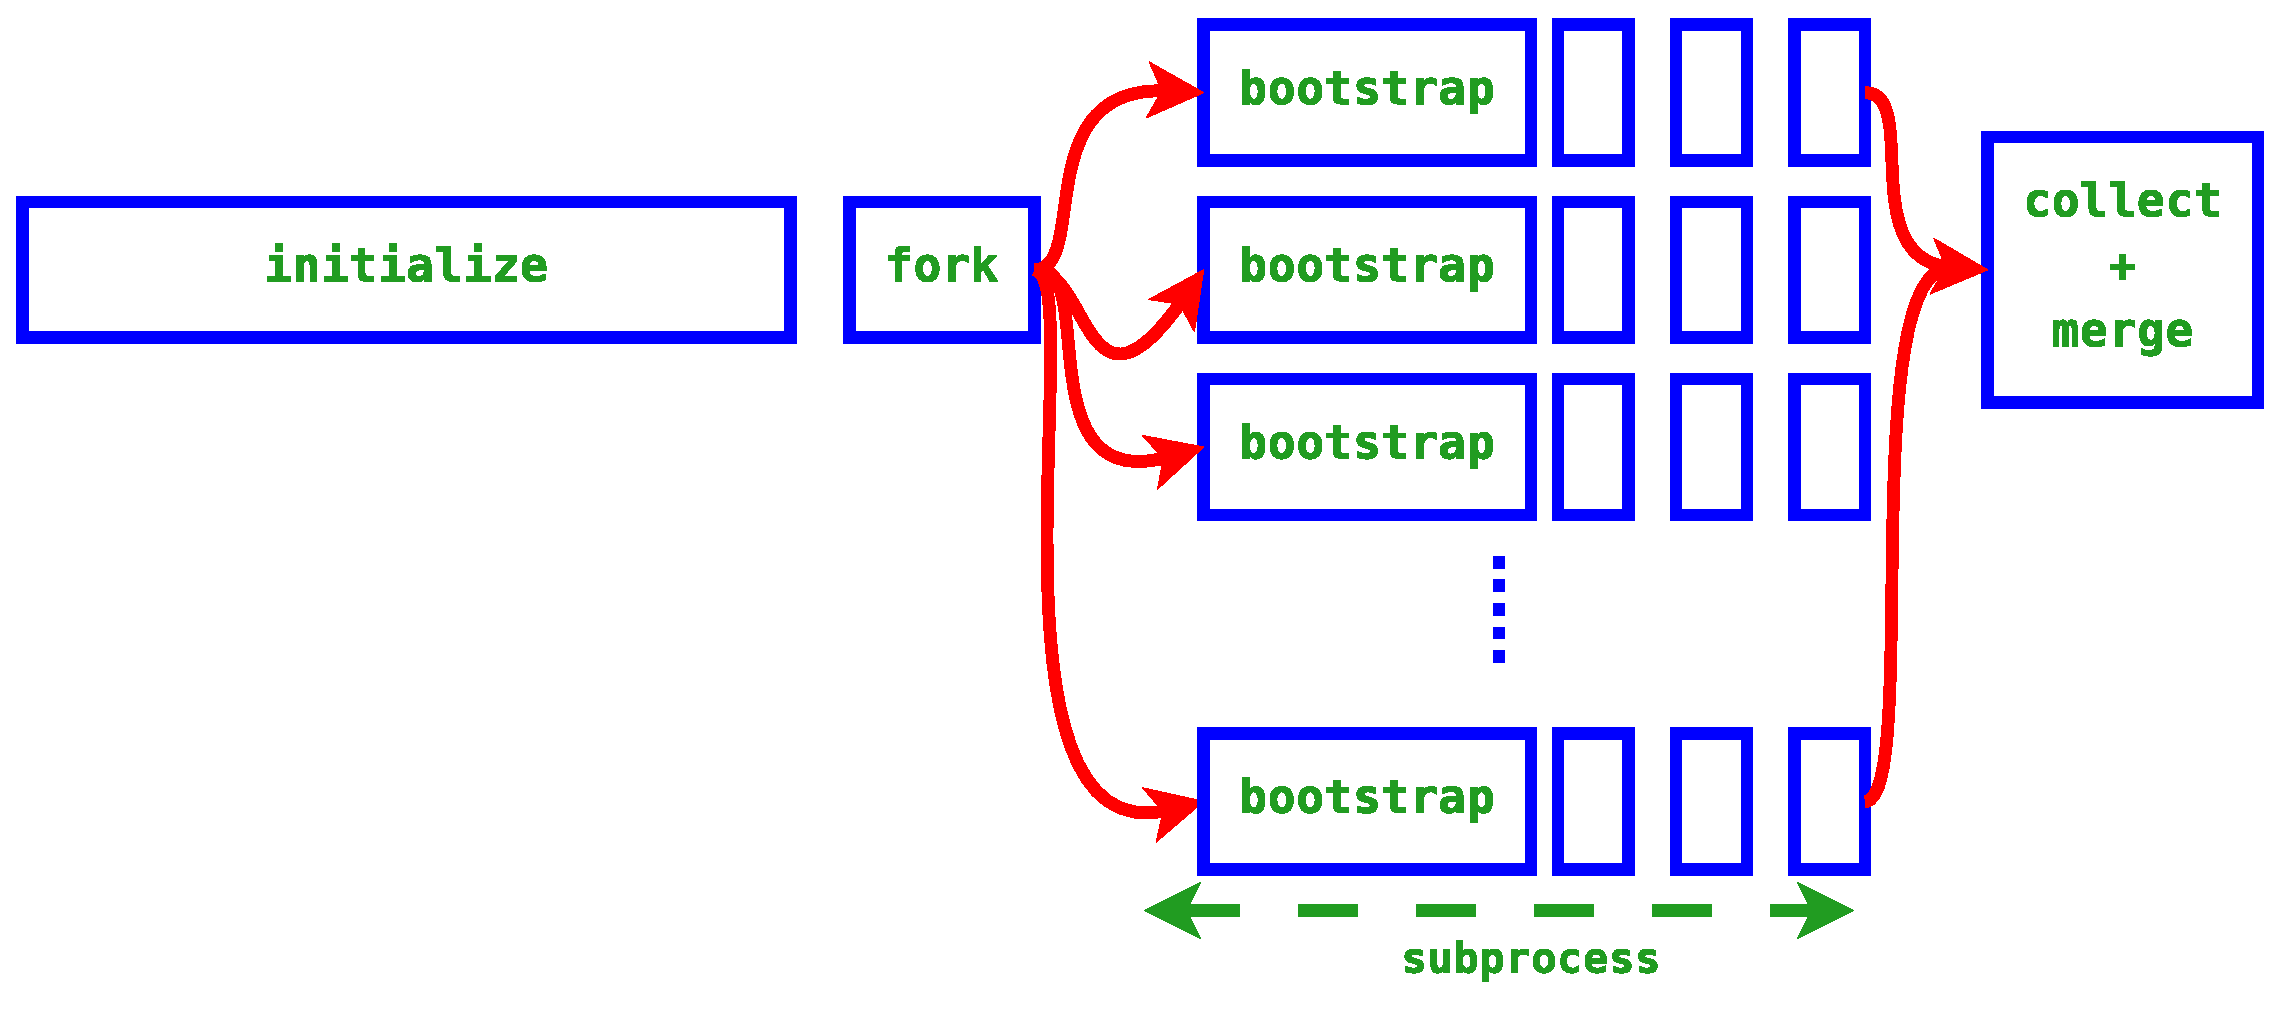
\includegraphics[angle=0,width=0.7\textwidth]{figs/athenamp-sequence.eps}
    \end{center}
  \end{figure}
}

\frame{
  \frametitle{\texttt{AthenaMP}}

  \begin{columns}
    \begin{column}{0.9\textwidth}

      \begin{block}{Impl\'ementation (S. Binet)}
        \begin{itemize}
          \item cr\'eation d'un nouveau event loop manager: \texttt{MpEventLoopMgr}
            \begin{itemize}
              \item encapsulation des d\'etails MP
              \item activation/d\'esactivation \emph{via} joboptions
            \end{itemize}
          \item utilisation d'un module \texttt{python} (\mygreen{\texttt{multiprocessing}}, dans la librairie standard de py-2.6) pour la gestion des sous-processus
            \begin{itemize}
              \item \emph{pool} de sous-processus ($= ncores$)
              \item gestion des fichiers d'entr\'ee et de sortie
            \end{itemize}
          \item cr\'eation d'un script pour \emph{merger} les fichiers POOL et ROOT
            \begin{itemize}
              \item de loin la partie la plus d\'elicate (POOL, \texttt{ElementLink}s, \ldots)
            \end{itemize}
        \end{itemize}
      \end{block}

      \begin{exampleblock}{Status}
        \begin{itemize}
          \item \emph{alpha} code
          \item test\'e avec \texttt{rdotoesdnotrigger} et \texttt{esdtoaod}
          \item tourne \mygreen{{\bf OK}} mais tests plus approfondis n\'ecessaires
            \begin{itemize}
              \item d\'eveloppement des outils de validation \myred{en cours} (\mygreen{\texttt{PyDumper}})
            \end{itemize}
        \end{itemize}
      \end{exampleblock}
    \end{column}
  \end{columns}

}

\frame{
  \frametitle{R\'esultats pr\'eliminaires}

  \begin{columns}
    \begin{column}{0.95\textwidth}

      \begin{exampleblock}{cpu - \texttt{RecExCommon/esdtoaod}}
        \texttt{4procs  242.85s user 8.71s system 249\% cpu 1:40.99 total}\\
        \texttt{3procs  213.67s user 7.30s system 191\% cpu 1:55.12 total}\\
        \texttt{2procs  181.67s user 6.13s system 149\% cpu 2:05.77 total}\\
        \texttt{1procs  162.52s user 5.22s system 093\% cpu 2:59.18 total}\\
        \texttt{0procs  160.25s user 4.28s system 094\% cpu 2:53.45 total}\\
      \end{exampleblock}
    \end{column}
  \end{columns}

 \begin{figure}
    \begin{center}
      \includegraphics[angle=0,width=0.6\textwidth]{figs/cpu.eps}
    \end{center}
  \end{figure}
}

\frame{
  \frametitle{R\'esultats pr\'eliminaires - II}

  \begin{columns}
    \begin{column}{0.95\textwidth}

      \begin{exampleblock}{memory - \texttt{RecExCommon/esdtoaod}}
        process: $\sim 700MB\ VMem$ and $\sim 420MB\ RSS$\\
        \texttt{(before) evt 0: private: 004 MB | shared: 310 MB}\\
        \texttt{(before) evt 1: private: 235 MB | shared: 265 MB}\\
        \ldots\\
        \texttt{(before) evt50: private: 250 MB | shared: 263 MB}
      \end{exampleblock}
    \end{column}
  \end{columns}

 \begin{figure}
    \begin{center}
      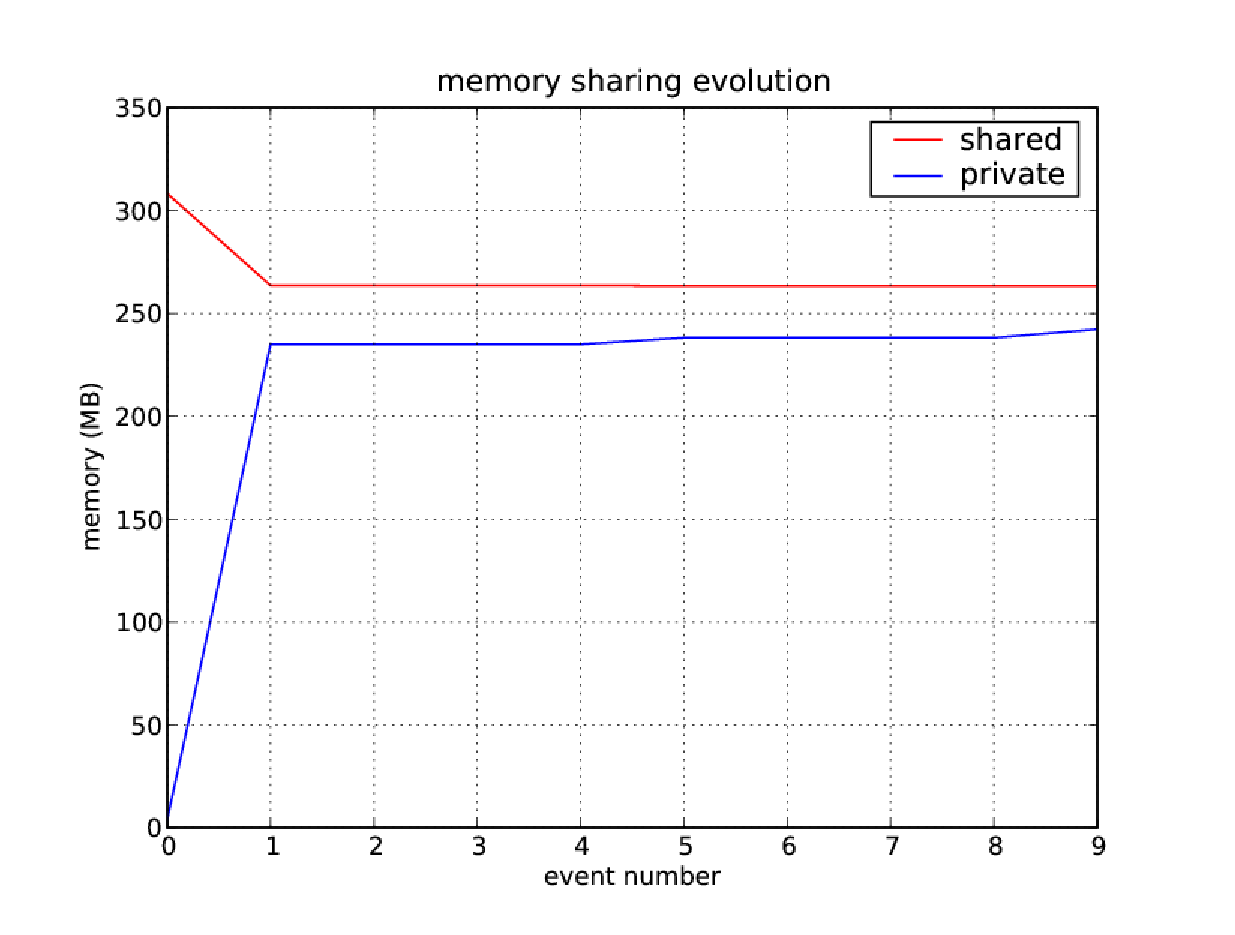
\includegraphics[angle=0,width=0.6\textwidth]{figs/vmem-share.epsi}
    \end{center}
  \end{figure}
}

\frame{
  \frametitle{Prospects}

  \begin{columns}
    \begin{column}{0.7\textwidth}
      \begin{block}{}
        \begin{itemize}
          \item d\'eveloppement d'un prompt interactif \myred{et} \emph{MP}
            \begin{itemize}
              \item \`a la \texttt{PROOF}
              \item r\'eduction latence de l'analyse \emph{'laptop'}
            \end{itemize}
          \item d\'eploiement sur la grille
            \begin{itemize}
              \item simples utilisateurs
              \item production ?
              \item probl\`emes d'interoperabilit\'e avec les \emph{batch systems}
            \end{itemize}
        \end{itemize}
      \end{block}

      \begin{exampleblock}{}
        Plus de tests:
        \begin{itemize}
          \item backnavigation ($AOD\rightarrow ESD\rightarrow RDO$)
          \item physics plots
          \item random numbers reproduceability
          \item reproduceability
          \item debugging tools
          \item \ldots
        \end{itemize}
      \end{exampleblock}
    \end{column}
  \end{columns}
}

\frame{

  \begin{columns}
    \begin{column}{0.7\textwidth}
      \begin{block}{}
        \begin{center}
          Backup\ldots
        \end{center}
      \end{block}
    \end{column}
  \end{columns}
}

\frame{
  \frametitle{\texttt{AthenaMP} implementation}

  \begin{columns}
    \begin{column}{0.95\textwidth}

      \begin{block}{rational}
        \begin{itemize}
          \item avoid client changes
          \item shove the MP-stuff \myred{inside} \texttt{Athena} instead of putting it as a layer on top of it
          \item use the \texttt{python} module \mygreen{\texttt{multiprocessing}} (backported from 2.6) for the process management
          \item write a new event loop manager as a usual \texttt{Gaudi} component to encapsulate the parallelism handling
          \item modify the I/O-related components appropriately
        \end{itemize}
      \end{block}

    \end{column}
  \end{columns}
}

\begin{frame}[fragile]{}

  \begin{columns}
    \begin{column}{0.95\textwidth}

\begin{python}
class MpEventLoopMgr (PyAthena.Svc):
    def executeRun (self, maxevt):
        """Process `maxevt` events as Run (beginRun->endRun)
        """
        if self._ncpus <= 0:
            return self._evtloop_mgr.executeRun (maxevt)

        import multiprocessing as mp
        _info ("nbr of workers: %i", self._ncpus)
        _info ("master workdir: %s", self._wkdir)
        workers = mp.Pool (processes=self._ncpus,
                           initializer=self._worker_bootstrap)
        results = workers.map_async (func=batch_run,
                                     iterable=(maxevt,)*self._ncpus)
\end{python}

\begin{exampleblock}{\bf{\myred{\texttt{\_worker\_bootstrap}}}}
\begin{itemize}
  \item function called after \texttt{fork}
  \item change work dir
  \item reopen file descriptors
  \item tickle the \texttt{IoComponentMgr}
\end{itemize}
\end{exampleblock}
    \end{column}
  \end{columns}
\end{frame}

\begin{frame}[fragile]{}

  \begin{columns}
    \begin{column}{0.95\textwidth}

\begin{C++}
class IIoComponentMgr 
{
  /** allow a @c IIoComponent to register itself with this
   *  manager so appropriate actions can be taken when e.g.
   *  a @c fork(2) has been issued (this is usually handled
   *  by calling @c IIoComponent::io_reinit on every registered
   *  component)
   */
  virtual
  StatusCode io_register (IIoComponent* iocomponent) = 0;
  
  /** @brief: reinitialize the I/O subsystem.
   *  This effectively calls @c IIoComponent::io_reinit on all 
   *  the registered @c IIoComponent.
   */
  virtual
  StatusCode io_reinitialize () = 0;

  /** @brief: finalize the I/O subsystem.
   *  Hook to allow to e.g. give a chance to I/O subsystems to 
   *  merge output files.
   */
  virtual
  StatusCode io_finalize () = 0;
};
\end{C++}

    \end{column}
  \end{columns}
\end{frame}

\begin{frame}[fragile]{}

  \begin{columns}
    \begin{column}{0.95\textwidth}

\begin{C++}
class IIoComponent
{
  /** callback method to reinitialize the internal state of
   *  the component for I/O purposes (e.g. upon @c fork(2))
   */
  virtual
  StatusCode io_reinit () = 0;
};
\end{C++}

\begin{block}{}
\begin{itemize}
  \item implemented by \texttt{THistSvc}, \texttt{AthenaPoolSvc}, \ldots
  \item reopen input ROOT files
  \item open output ROOT files
    \begin{itemize}
      \item created in the worker's own directory
      \item take care of migrating all the objects of \emph{'already opened for writting'} ROOT files to the new ones
    \end{itemize}
\end{itemize}
\end{block}

    \end{column}
  \end{columns}
\end{frame}

\begin{frame}[fragile]{}

  \begin{columns}
    \begin{column}{0.95\textwidth}

\begin{python}
class MpEventLoopMgr (PyAthena.Svc):
    def executeRun (self, maxevt):
        """Process `maxevt` events as Run (beginRun->endRun)
        """
        if self._ncpus <= 0:
            return self._evtloop_mgr.executeRun (maxevt)

        import multiprocessing as mp
        _info ("nbr of workers: %i", self._ncpus)
        _info ("master workdir: %s", self._wkdir)
        workers = mp.Pool (processes=self._ncpus,
                           initializer=self._worker_bootstrap)
        results = workers.map_async (func=batch_run,
                                     iterable=(maxevt,)*self._ncpus)
\end{python}

\begin{block}{\bf{\mypurple{\texttt{batch\_run}}}}
\begin{itemize}
  \item inject a filter algorithm in front of alg-sequence
    \begin{itemize}
      \item accept/reject events based on local process-id and current event number
    \end{itemize}
  \item effectively implement a round-robin filter
  \item call the \myred{\texttt{executeRun}} of the wrapped event loop manager
\end{itemize}
\end{block}
    \end{column}
  \end{columns}
\end{frame}

\begin{frame}[fragile]{}

  \begin{columns}
    \begin{column}{0.95\textwidth}

\begin{python}
class MpEventLoopMgr (PyAthena.Svc):
    def finalize (self): ...
\end{python}

\begin{block}{}
\begin{itemize}
  \item tickle \myred{\texttt{IIoComponentMgr::io\_finalize}} (when a forked process)
  \item master will run the merge of output files
    \begin{itemize}
      \item usually trivial for ROOT files containing histos and ntuples
      \item trickier for ROOT/POOL files
        \begin{itemize}
          \item take care of POOL links/references
          \item actually just a few integers here and there to offset by the right amount
          \item needs some modifications in the \texttt{AthenaPOOL} layer to enable usage of the fast-merge mode (\emph{\`a la} \texttt{hadd})
          \item right now: pedestrian/manual approach (slower)
        \end{itemize}
      \item \mygreen{I wish there were a general \texttt{pool\_merge} command !}
    \end{itemize}
\end{itemize}
\end{block}
    \end{column}
  \end{columns}
\end{frame}

\end{document}


